\documentclass[12pt,a4paper]{scrartcl}
\renewcommand{\baselinestretch}{1.359141}
% scrartcl ist eine abgeleitete Artikel-Klasse im Koma-Skript
% zur Kontrolle des Umbruchs Klassenoption draft verwenden


% die folgenden Packete erlauben den Gebrauch von Umlauten und ß
% in der Latex Datei
\usepackage[utf8]{inputenc}
\usepackage[T1]{fontenc}
\usepackage[ngerman]{babel}


\usepackage[pdftex]{graphicx}
\usepackage{latexsym}
\usepackage{amsmath,amssymb,amsthm}
\usepackage{xcolor}
\usepackage{tikz}
\usepackage{pgfplots}
\usepackage{mhchem}
\usepackage{braket}
\usepackage{hyperref}
\usetikzlibrary{scopes}


% Abstand obere Blattkante zur Kopfzeile ist 2.54cm - 15mm
\setlength{\topmargin}{-15mm}


% Umgebungen für Definitionen, Sätze, usw.
% Es werden Sätze, Definitionen etc innerhalb einer Section mit
% 1.1, 1.2 etc durchnummeriert, ebenso die Gleichungen mit (1.1), (1.2) ..
\newtheorem{Satz}{Satz}[section]
\newtheorem{Definition}[Satz]{Definition}
\newtheorem{Lemma}[Satz]{Lemma}

\numberwithin{equation}{section}

\begin{document}
  % Keine Seitenzahlen im Vorspann
  \pagestyle{empty}

  % Titelblatt der Arbeit
  \begin{titlepage}

    \vspace*{2cm}

 \begin{center} \large

    Seminararbeit
    \vspace*{2cm}

    {\huge Asymmetrien der Physik}
    \vspace*{2.5cm}

    Matteo Schmider
    \vspace*{1.5cm}

    05.11.2019
    \vspace*{4.5cm}


    Betreuung: StR Johannes Klees \\[1cm]
    W-Seminar Wissenschaft und Comedy \\[1cm]
		Simpert-Kraemer Gymnasium Krumbach
  \end{center}
\end{titlepage}



  % Inhaltsverzeichnis
  \tableofcontents

\newpage



  % Ab sofort Seitenzahlen in der Kopfzeile anzeigen
  \pagestyle{headings}

  \section{Einleitung: Super-Asymmetrie und die reale Physik}

Erst vor kurzem strahlte der deutsche Fernsehsender ProSieben die letzte Staffel der Serie \glqq{The Big Bang Theory}\grqq{} aus. Bekanntermaßen handelt die Serie von der WG der beiden fiktiven Physiker Dr. Leonard Leakey Hofstadter und Dr. Dr. Sheldon Lee Cooper und ihrem \glqq{Nerd-Dasein}\grqq{}, das im starken Widerspruch zum Charakter ihrer Nachbarin, Penny steht. Die Serie ist unter anderem für die vielen, oft komödiantischen, Anspielungen auf reale physikalische Phänomene und Theorien bekannt. Ihren Höhepunkt erreicht sie jedoch in ihrer letzten Folge, deren Hauptinhalt die Nobelpreisverleihung an Sheldon und seine Freundin Amy für ihre Theorie der Super-Asymmetrie bildet. In dieser Arbeit möchte ich einen Einblick in die Bedeutung von Symmetrien und Asymmetrien in der Physik geben, anhand des erstaunlichen Phänomens der indirekten T-Verletzung. Die T-Verletzung ist eine Schlussfolgerung aus der experimentell nachgewiesenen CP-Verletzung und der Gültigkeit der CPT-Theorie, wobei deren Verletzungen historisch als unmöglich betrachtet wurden. Das CPT-Theorem ist trotz der unglaublich interessanten und verblüffenden Folgerungen und Beobachtungen, die sich daraus ergeben, kein sehr bekannter Bestandteil der modernen Physik. Daher ist es auch ein Ziel dieser Arbeit, dem Leser eine der vielen kleinen Forschungsthemen der Physik nahe zu bringen, die außerhalb eines kleinen Fachkreises wenig Aufmerksamkeit finden.

%%%%%%%%%%%%%%%%%%%%%%%%%%%%%%%%%
  \newpage  % neuer Abschnitt auf neue Seite, kann auch entfallen
%%%%%%%%%%%%%%%%%%%%%%%%%%%%%%%%%

  \section{Allgemeine Transformation einer physikalischen Größe}

Eine Transformation f einer physikalischen Größe x ist im Allgemeinen immer eine Abbildung der Art
\begin{align}
    f: x \to x'
\end{align}
Als sehr simples Beispiel könnte man eine Transformation f definieren, die ein physikalisches System in eines umwandelt, in dem alle Massen verdoppelt sind:
\begin{align}
    f(m) = 2m
\end{align}
Diese Transformation ist zwar sehr anschaulich, aber leider nicht sehr nützlich. Eine deutlich gebräuchlichere Transformation der modernen Physik findet sich in der Lorentz-Transformation:
\begin{align}
  \begin{split}
    t' &= \gamma(t - \frac{v_x}{c^2}x) \\ x' &= \gamma(x -v_x t) \\ y' &= y \\ z' &= z \\ v_x' &= -v_x
  \end{split}
\end{align}
Diese Transformation beschreibt, wie ein Inertialsystem A am Ort $ \vec{r} = \begin{pmatrix}x\\y\\z\end{pmatrix} $, mit konstanter Geschwindigkeit $v_x$ in x-Richtung relativ zum Beobachter-System B, zur Zeit t' und B ineinander überführt werden kann. Die Lorentz-Transformation ist für die relativistische Raumzeit gültig und ersetzt darin die Galilei-Transformation. Diese Transformation ist daher auch für relativistische Systeme gültig, weswegen sie heute noch viel verwendet wird. Dieses Beispiel soll nur zeigen, dass Transformationen nichts Neues in der Physik sind, und als nützliche Hilfsmittel immer wieder Verwendung finden.
Wichtig für den weiteren Verlauf der Arbeit ist jedoch vor allem die grundlegende Transformation der Spiegelung:
\begin{align}
    f: x \to - x'
\end{align}
Diese Transformation sieht sehr simpel aus und wie mehrmals in dieser Arbeit zu sehen sein wird, hat diese Transformation zumeist auch keinen großen Effekt. Wenn nun nämlich eine Größe auf ihre Symmetrie gegnüber der SPiegelung geprüft weren soll, man nehme an, diese wäre durch die Funktion $x(t) = t^2$ bestimmt. Nun kann diese Größe einer Zeit-Spiegelung unterzogen werden, die die Form $T(t) = -t$ hat, und erhält $x(T(t)) = (-t)^2$. Damit ist offensichtlich, dass sich das Verhalten der Größe gar nicht ändert. Eine Größe ist immer dann symmetrisch unter einer Transformation, wenn das Ergebnis dasselbe oder das exakte Inverse der Ausgangslage ist. Tatsächlich ist die Prämisse hinter den folgenden Überlegungen, diese Symmetrien selbst als Naturgesetz aufzugreifen und zu kategorisieren.

%%%%%%%%%%%%%%%%%%%%%%%%%%%%%%%%%
  \newpage  % neuer Abschnitt auf neue Seite, kann auch entfallen
%%%%%%%%%%%%%%%%%%%%%%%%%%%%%%%%%

  \section{C-Transformation und C-Invarianz}

Die CPT-Symmetrie besteht aus drei einzelnen Symmetrien, die im Folgenden erst einmal einzeln erläutert werden, beginnend mit der C-Symmetrie. \\
Die C-Transformation hat ihren Namen von \glqq{charge}\grqq{} (engl. Ladung) und \glqq{spiegelt}\grqq{} die Ladung eines betrachteten Teilchens. Nachdem Elementarteilchen eine feste Ladung besitzen, ist diese Operation in der Realität als das Ersetzen des Teilchens durch das dazugehörige Antiteilchen zu verstehen. Das Antiteilchen besitzt immer dieselbe Masse und Eigenschaften des Ausgangs-Teilchens, bis auf die \glqq{umgedrehte}\grqq{} Ladung. Eine Invarianz unter dieser Symmetrie bedeutet, dass sich physikalische Systeme, die durch die C-Transformation transformiert wurden, sich genauso verhalten wie deren nicht-transformierte Variante. Ein guter Weg sich vorzustellen, woraus sich diese Invarianz ergibt, ist, ein Beispiel zu betrachten, das sich nicht invariant darunter verhält. Dazu betrachte man zwei stark vereinfachte Teilchen, die dieselbe Masse und positive Ladung besitzen und eine Längeneinheit voneinander entfernt liegen. Nun ist sehr offensichtlich, dass sich aufgrund der gleichen Ladungen nach dem coulombschen Gesetz die Ladungen direkt voneinander weg bewegen. Ebenso nach dem coulombschen Gesetz sollten beide Teilchen dieselbe Kraft dabei erfahren.\cite{shnirman15}
\begin{figure} [!ht]
\centering
\begin{tikzpicture}[
      force/.style={>=latex,draw=blue,fill=blue},
      axis/.style={densely dashed,gray,font=\small},
      m/.style={circle,draw=black,fill=blue,minimum size=0.6cm,thick}
]
      \node[m] at (1, 0) (m1) {};
      {[force,->]
          \draw (m1.east) -- ++(1,0) node[above] {F\textsubscript{1}};
      }
      \node[m] at (-1, 0) (m2) {};
      {[force,->]
          \draw (m2.west) -- ++(-1,0) node[above] {F\textsubscript{2}};
      }
\end{tikzpicture}
\begin{align}
    \lvert F\textsubscript{1}\rvert\ = \lvert F\textsubscript{2}\rvert\
\end{align}
\caption{Das Beispiel vor der Transformation}
\end{figure}
\\
Nach der C-Transformation ist der Startzustand derselbe, mit dem Unterschied, dass die Ladungen negativ sind. Die Teilchen wurden durch ihre Antiteilchen ersetzt. Eine Invarianz unter der C-Transformation würde dasselbe Verhalten aufweisen, wie der zuvor besprochene Vorgang. Da jedoch in diesem Beispiel die Symmetrie gebrochen werden soll, kann man den Teilchen zufällig Richtung und Betrag der Kräfte zuordnen, da eben nicht dieselben physikalischen Gesetze wie in der nicht-transformierten Welt gültig sind.
\\
\begin{figure} [!ht]
\centering
\begin{tikzpicture}[
      force/.style={>=latex,draw=blue,fill=blue},
      axis/.style={densely dashed,gray,font=\small},
      m/.style={circle,draw=black,fill=blue,minimum size=0.6cm,thick}
]
      \node[m] at (1, 0) (m3) {};
      {[force,->]
          \draw (m3.west) -- ++(-0.5,0) node[above] {F\textsubscript{3}};
      }
      \node[m] at (-1, 0) (m4) {};
      {[force,->]
          \draw (m4.east) -- ++(0.25,0) node[above] {F\textsubscript{4}};
      }
\end{tikzpicture}
\begin{align}
    \lvert F\textsubscript{1}\rvert = \lvert F\textsubscript{2}\rvert \neq \lvert F\textsubscript{3}\rvert \neq \lvert F\textsubscript{4}\rvert
\end{align}
\caption{Nach der Transformation, mit gebrochener Symmetrie}
\end{figure}
Das hierdurch dargestellte System entspricht natürlich überhaupt nicht unserem gewohnten Verständnis von dem Verhalten elektronischer Ladungen. Ersichtlich ist damit auch, dass das coulombsche Gesetz selbst invariant unter der C-Transformation ist und sein Verhalten nicht umdreht, wenn die Ladung das Vorzeichen wechselt, weswegen es in diesem willkürlichen Beispiel auch nicht mehr gilt.
\\
In der CPT-Theorie geht man nun davon aus, dass die C-Symmetrie nie gebrochen wird, also alle Prozesse unabhängig von dem Vorzeichen der Ladung funktionieren, also nur auf Ladungsunterschieden beruhen. Hiermit lässt sich auch begründen, dass die Wahl von + und - für die Teilchen des Standardmodells vollkommen willkürlich ist. Die Physiker hätten sich genauso darauf einigen können, dass das Elektron eine positive und Protonen eine negative Ladung besitzen, und dementsprechend Ladungen angegeben würden, ohne das sich eine einzige Gleichung dafür ändern müsste. Die Invarianz hat auch zur Folge, dass Materie und Antimaterie sich nicht in ihrem Verhalten unterscheiden. Die Wahl des Begriffs Materie für die uns bekannte und Antimaterie für deren Antiteilchen ist also ebenso willkürlich gewählt.\cite{lueders54}

%%%%%%%%%%%%%%%%%%%%%%%%%%%%%%%%%
  \newpage  % neuer Abschnitt auf neue Seite, kann auch entfallen
%%%%%%%%%%%%%%%%%%%%%%%%%%%%%%%%%

  \section{P-Transformation und P-Invarianz}

Die P-Transformation findet sich deutlich häufiger in unserem Alltag und sollte damit wohl am einfachsten zu verstehen sein. P steht für parity oder Parität und bezeichnent die Invarianz unter räumlicher Spiegelung. Parität tritt in zwei unterschiedlichen Formen auf: positiv und negativ. Eine positive Parität liegt dann vor, wenn ein System nach seiner räumlichen Spiegelung in einer seiner Größen denselben Wert behält, eine negative, wenn der Wert das jeweils andere Vorzeichen besitzt. Wenn also eine Größe eine negative Parität hat, so könnte man ebenso sagen, dass der Betrag der Größe einer positiven Parität unterliegt. Der allgemeine Begriff der Parität bezieht sich auf jegliche Transformation der Koordinaten eines Systems. Üblicherweise ist die P-Transformation des CPT-Theorems jedoch eine Spiegelung in allen drei Koordinatenachsen, also eine Punktspiegelung.
\begin{figure} [!ht]
\centering
\begin{tikzpicture}
\begin{axis}[
  view={35}{15},
  axis lines=center,
  width=16cm,height=9cm,
  xmin=-4,xmax=4,ymin=-2,ymax=2,zmin=-2,zmax=2
]
% plot dots for the two points
\addplot3 [only marks] coordinates {(1,1,1) (3,1,1)};
% label points
\node [above right] at (axis cs:1,1,1) {A};
\node [above left] at (axis cs:3,1,1) {B};
\draw [->, thick] (axis cs:1,1,1) -- (axis cs:1.75,1,1);
\draw [->, thick] (axis cs:3,1,1) -- (axis cs:2.25,1,1);
\node [below] at (axis cs:1,1,1) {$\vec{F}\textsubscript{1}$};
\node [below] at (axis cs:3,1,1) {$\vec{F}\textsubscript{2}$};
\end{axis}
\end{tikzpicture}
\caption{Vor der Punktspiegelung}
\end{figure}
\\
Die P-Transformation lässt sich sehr einfach veranschaulichen: In Abbildung 3 ist der Startzustand dargestellt, Abbildung 4 zeigt die die gespiegelte Version. Nun nehme man an, dass sich in den Punkten A und B Objekte derselben Masse befinden und die Schwerkraft hier durch die Newton'sche Gravitation angenähert wird (anstelle der Einstein'schen Gravitation), also durch die Beziehung
\begin{align}
  \vec{F}\textsubscript{1} = -\vec{F}\textsubscript{2} = G\frac{m\textsubscript{1}m\textsubscript{2}}{r^3}\vec{r}\textsubscript{1,2}
\end{align}
gegeben ist. Die Beträge dieser gerichteten Kräfte sind im Allgemeinen bekannt als
\begin{align}
  {F}\textsubscript{1} = {F}\textsubscript{2} = G\frac{m\textsubscript{1}m\textsubscript{2}}{r^2}
\end{align}
Hier lässt sich schon direkt erkennen, dass die Beträge von der Gravitationskonstanten G, den nicht veränderten Massen m\textsubscript{1} und m\textsubscript{2}, sowie dem Quadrat des Abstands abhängig sind. Alle diese Größen sind von einer simplen Spiegelung nicht betroffen. Daher ist die Gravitation negativer Parität, nachdem sich die Richtungen der Vektoren umkehren und der Betrag unbetroffen von der Spiegelung bleibt.\cite{leeyang56, lueders54}
\begin{figure} [!ht]
\centering
\begin{tikzpicture}
\begin{axis}[
  view={35}{15},
  axis lines=center,
  width=16cm,height=9cm,
  xmin=-4,xmax=4,ymin=-2,ymax=2,zmin=-2,zmax=2
]
% plot dots for the two points
\addplot3 [only marks] coordinates {(-1,-1,-1) (-3,-1,-1)};
% label points
\node [above right] at (axis cs:-1,-1,-1) {A};
\node [above left] at (axis cs:-3,-1,-1) {B};
\draw [->, thick] (axis cs:-1,-1,-1) -- (axis cs:-1.75,-1,-1);
\draw [->, thick] (axis cs:-3,-1,-1) -- (axis cs:-2.25,-1,-1);
\node [below] at (axis cs:-1,-1,-1) {$\vec{F}'\textsubscript{1}$};
\node [below] at (axis cs:-3,-1,-1) {$\vec{F}'\textsubscript{2}$};
\end{axis}
\end{tikzpicture}
\caption{nach der Punktspiegelung}
\end{figure}

%%%%%%%%%%%%%%%%%%%%%%%%%%%%%%%%%
  \newpage  % neuer Abschnitt auf neue Seite, kann auch entfallen
%%%%%%%%%%%%%%%%%%%%%%%%%%%%%%%%%

  \section{T-Transformation und T-Invarianz}

Die T-Transformation und T-Invarianz stellen den letzten Teil des CPT-Theorems. T steht für \glqq{time}\grqq{} (engl. Zeit) und meint die Umkehrung der Zeitrichtung. Diese Transformation wird in einigen Quellen auch als Bewegungsumkehr \cite{wigner32} bezeichnet, da natürlich vor allem die einfach polynomisch/linear von der Zeit abhängigen Größen (wie die Geschwindigkeit) von der T-Transformation betroffen und gleichzeitig leicht verständlich sind. Konkret vorstellen kann man sich diese Transformation als das rückwärts Abspielen eines Films. Die T-Invarianz bedeutet nun, dass beim Rückwärtsabspielen alle Beträge der Geschwindigkeiten gleich bleiben, das ein rückwärts abgespielter Film also exakt so lange zum Ansehen benötigt, wie ein vorwärts abgespielter. Diese Annahme war schon lange vor ihrer Formalisierung im CPT-Theorem quasi unterbewusst in der Physik bekannt. Ein gutes Beispiel dafür ist das bekannte Fadenpendel: Solange Reibungseffekte vernachlässigt werden, schwingt ein Pendel immer von rechts nach links und wieder zurück. Die Auslenkung nimmt die Form einer Kosinus-Kurve an (siehe Abbildung 5). Da die Periode abhängig ist vom Gewicht des Pendels, sowie der Fadenlänge und der lokalen Erdanziehung, ändert sich die Periode nicht durch die Zeitumkehr. Nachdem die Zeitumkehr als Funktion T mit
\begin{align}
  T: t \to - t
\end{align}
dargstellt werden kann, lässt sich der Graph für die Auslenkung auch für die zeitumgekehrte Version darstellen, die sich durch ersetzen der Zeit t durch die Transformierte ergibt:
\begin{align}
  A(t) = cos(t)
  A'(t) = cos(T(t)) = cos(-t) = cos(t)
\end{align}
Nachdem cos(-t) = cos(t) stellt sich heraus, das beim Umkehren der Zeit sich das System in keinster Weise verändert. \\
Der einzige Teil der klassischen Mechanik (in dem vorangegangenen Beispiel daher nicht beachtet), der nicht invariant unter Zeitumkehr ist, ist die Reibung, die sich immer gegen eine Bewegung richtet, und daher bei der Zeitumkehr eine Bewegung \glqq{aus dem Nichts}\grqq{} heraus beschleunigen müsste. Dieser Effekt macht tatsächlich Sinn, nachdem die dafür nötige Energie in Form von mehr Wärme, die zuvor bei der Reibung erzeugt wurde vorhanden wäre. Allerdings würde das Umwandeln von Wärmeenergie in kinetische Energie auf so eine geordnete Art und Weise entgegen der Thermodynamik. Als Beispiel dafür kann man sich ein Glas vorstellen, das von einem Tisch fällt und zerbricht. Durch das Zerbrechen entsteht Unordnung, es entstehen mehr individuelle Teile, die sich über eine größere Fläche auf dem Boden verteilen, etc. Dieses Verhalten wird als physikalisch wahrscheinlich betrachtet, das Universum \glqq{will}\grqq{}, dass mehr Unordnung entsteht, es begünstigt mit der Gravitaion das Herunterfallen und Zerbrechen des Glases. Diese Eigenschaft äußert sich nun in dem zweiten Gesetz der Thermodynamik \cite{pfennig12}, nach dem sich die Entropie, eine Maßeinheit für die Unordnung mit zunehmender Zeit erhöht. Damit wäre die Zeitsymmetrie gebrochen, und unsere Erfahrung von einer einzigen Zeitrichtung bestätigt. Denn wenn sich die Entropie stetig erhöht, könnte man zwei beliebige Zeitpunkte betrachten, das ganze Glas auf dem Tisch und das zerbrochene auf dem Boden, und immer eindeutig daraus schließen, das der Zustand, in dem das Glas zerbrochen ist aufgrund der höheren Entropie zeitlich später als der Zustand in dem das Glas noch ganz ist, sein muss. Leider ist die Größe der Entropie rein statistischer Natur, und nur für makroskopische Systeme mit vielen Milliarden von Abermilliarden an Teilchen gültig. In einem System mit nur wenigen Teilchen ist solch eine Schlussfolgerung nahezu unmöglich. Doch nachdem diese großen Systeme eben aus vielen kleinen Teilchen-Systemen bestehen, muss der Vorgang tatsächlich auch dort reversibel sein. Die Zeitumkehr scheint in diesem Beispiel fast unmöglich, ein zerfallenes Glas, dass sich wider auf den Tisch bewegt, und sich dabei wieder zusammensetzt sollte doch jeglicher Logik widersprechen. Doch wenn jedes Teilchen einzeln betrachtet und deren Wege zurückverfolgt werden, dann macht die Zeitumkehr tatsächlich physikalisch Sinn, wäre sogar exakt berechenbar. Die Zeitsymmetrie wird hier also nicht fundamental gebrochen, sondern ist ein rein statistisches Phänomen, das nur auf makroskopischer Ebene auftritt.\cite{aue08}

%%%%%%%%%%%%%%%%%%%%%%%%%%%%%%%%%
  \newpage  % neuer Abschnitt auf neue Seite, kann auch entfallen
%%%%%%%%%%%%%%%%%%%%%%%%%%%%%%%%%

  \section{Zusammenhang zwischen C, P und T}

Nachdem Anfang des 20. Jahrhunderts diese Symmetrien einzeln schon formalisiert wurden, kam nun eine weitere Frage auf: Gibt es ebenso Invarianzen unter Symmetrie-Kombinationen? Es lässt sich ja zumindest mathematisch sehr gut überprüfen, ob eine bestimmte Gleichung auch invariant unter der Hintereinanderausführung von Symmetrien ist. Es ist sehr schwierig, einer Person diese Überprüfungen zuzuordnen, doch ich möchte hierin vor allem auf die Arbeit von Gerhart Lüders eingehen, der zur Mitte des letzten Jahrhunderts aktiv dazu forschte. Es stellte sich nämlich in seiner Arbeit heraus, dass sich eine Art \glqq{höhere}\grqq{} Symmetrie aus den einzelnen dreien bilden lässt. Lüders bewies nämlich 1954, dass die Quantenmechanik, spezifischer jede relativistische Wellenfunktion, die den Anforderungen der Quantenmechanik genügt, auch invariant unter der CPT-Transformation ist. Die CPT-Transformation meint das Hintereinanderausführen einer C-, P- und T-Transformation, also das Ersetzen jeden Teilchens durch sein Antiteilchen, das räumliche Spiegeln und das Umkehren der Zeitrichtung zusammen. Diese höhere Symmetrie ist nicht nur eine Folgerung aus dem Kombinieren der Bestandteile, sondern eine eigene, davon unabhängige. Es könnte nämlich jede einzelne der drei Symmetrien verletzt sein, und trotzdem symmetrisch unter der CPT-Symmetrie als ganzem. Dazu müsste, nehme man an die C-Invarianz wäre gebrochen, \glqq{nur}\grqq{} das darauffolgende Ausführen der P- und T-Transformation diese Verletzung aufheben. Eine besondere Beziehung wird dadurch auffällig: Wenn eine der drei Symmetrien verletzt sein sollte, so muss, wenn die CPT-Symmetrie erhalten bleibt, die Kombination der zwei anderen Transformationen ebenso deren Invarianz verletzen. Wäre nun die C-Invarianz verletzt, so müssen die anderen beiden Transformation diese aufheben. Wenn nun jedoch die PT-Transformation die Symmetrie erhält, so würde sie die C-Verletzung ja nicht beheben können, da sie eben selbst symmetrisch wäre. \cite{lueders54} \\
Die Serie \glqq{The Big Bang Theory}\grqq{}, um die Einleitung wieder aufzugreifen, hat ihren Namen ja von der Urknalltheorie. Dieser Urknall hängt mit dem CPT-Theorem eng zusammen, denn es liegt die Annahme nahe, dass der Urknall eine Art Nullpunkt/Ursprung für die Zeit darstellt. Nun ließe sich ja argumentieren, dass die Physik invariant unter der CPT-Transformation ist, und daher ebenso gültig wäre in einem Universum, das räumlich zu unserem gespiegelt ist, dessen Materie wir als Antimeterie bezeichnen würden und dessen Zeit zu unserer verglichen rückwärts liefe. Wenn nun der Urknall den Ursprung bildet, von dem weg sich alles entwickelt, so könnte sich auf der anderen Seite dieses Ursprungs eine Art Anti-Universum befinden, das unserem exakt entspricht, bis auf die Veränderungen durch eine CPT-Transformation. Bildlich ließe sich das darstellen wie in Abbildung 5, und es zählt zu einem der möglichen Ansätze der modernen Physik, die Urknalltheorie zu begründen. \cite{schirber18}
\begin{figure} [!ht]
  \centering
  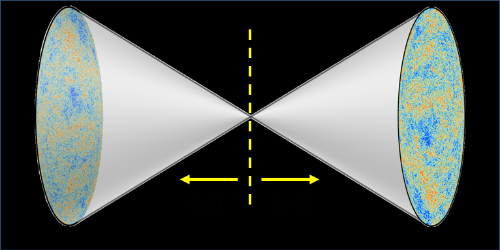
\includegraphics{antiuniverse}
  \caption{Ausbreitung der Raumzeit vor und nach dem Urknall}
\end{figure}

%%%%%%%%%%%%%%%%%%%%%%%%%%%%%%%%%
  \newpage  % neuer Abschnitt auf neue Seite, kann auch entfallen
%%%%%%%%%%%%%%%%%%%%%%%%%%%%%%%%%

  \section{Paritätsverletzung}

Bevor ich zum Finale all dieser doch recht theoretischen Überlegungen komme und die CP-Verletzung aufgreife, sollte jedoch zuerst die Entdeckung der P-Verletzung erwähnt werden. Bisher schienen ja alle Symmetrien und Invarianzen fest in unserer alltäglichen Welt verankert oder zumindest hinreichend logische Annahmen gewesen zu sein. Auf mikroskopischster Ebene jedoch spekulierten die Physiker Tsung-Dao Lee und Chen Ning Yang schon 1956, dass eine der vier grundlegenden physikalischen Kräfte, die schwache Kernkraft, um exakt zu sein, die Parität verletzen könnte.\cite{leeyang56} R. T. Cox, C. G. McIlwraith und B. Kurrelmeyer stellten bei Experimenten mit radioaktiver $\beta$-Strahlung schon knapp drei Jahrzehnte zuvor die Paritätsverletzung fest. Nachdem sich damals jedoch niemand vorstellen konnte, dass die P-Symmetrie verletzt sein könnte, wurde dieser Bestandteil der Ergebnisse als bloßer Messfehler abgetan.\cite{coxkurrelmeyer28} Dasselbe prinzipielle Experiment, natürlich in einem modifizierten Aufbau ist heute als Wu-Experiment bekannt. Der Name stammt von der Physikerin Chien-Shiung Wu, die Lee's und Yang's These noch im selben Jahr bewies. In diesem Experiment wurde der $\beta$-Zerfall vom radioaktiven Cobalt-Isotop $\ce{^{60}_{27}Co}$ beobachtet, der unter anderem Elektronen ausstößt. Die Elektronen werden entlang der Spin-Achse der Atome gezählt, einmal in und einmal entgegen der Spin-Richtung. Da der Spin eine Art Drehimpuls darstellt, und somit ein axialer Vektor ist, ist er von der Punktspiegelung nicht betroffen. In Abbildung 6 sind die Cobalt-Atome vor und nach der Transformation dargestellt, sowie deren Spin-Richtung und die Richtung, in die Elektronen ausgesendet werden. Nun lassen sich drei Fälle unterscheiden: Entweder fliegen mehr Elektronen in Spin-Richtung, entgegen der Spin-Richtung oder gleich viele in beide Richtungen. Würden die Elektronen nun eher entgegen der Spin-Richtung fliegen, wie hier dargestellt, wäre die gespiegelte Version ebenso wie der Spin unbetroffen von der Spiegelung. Das entspräche jedoch einer Paritätsverletzung, da die Flugrichtung nicht das Vorzeichen wechselt, wie eigentlich von einer einfachen Bewegung zu erwarten wäre.
Die einzige Möglichkeit, dass hierbei nicht die Parität verletzt wird, ist, wenn die Elektronen in gleich großen Mengen in beide Richtungen das Cobalt-Atom verlassen.
\begin{figure} [!ht]
\centering
\begin{tikzpicture}
\begin{axis}[
  view={35}{15},
  axis lines=center,
  width=10cm,height=13cm,
  xmin=-2,xmax=2,ymin=-2,ymax=2,zmin=-3,zmax=2
]
% plot dots for the two points
\addplot3 [only marks] coordinates {(1,1,1) (-1,-1,-1)};
% label points
\node [above right] at (axis cs:1,1,1) {$\ce{^{60}_{27}Co}$};
\node [below left] at (axis cs:-1,-1,-1) {$\ce{^{60}_{27}Co}'$};
\draw [->, thick] (axis cs:1,1,1) -- (axis cs:1,1,2);
\draw [->, thick] (axis cs:-1,-1,-1) -- (axis cs:-1,-1,0);
\node [right] at (axis cs:1,1,2) {Spin};
\node [below left] at (axis cs:-1,-1,0) {$Spin'$};
\draw [->, dotted] (axis cs:1,1,1) -- (axis cs:1,1,0);
\draw [->, dotted] (axis cs:-1,-1,-1) -- (axis cs:-1,-1,-2);
\node [below right] at (axis cs:1,1,0) {$e_1^-$};
\node [below right] at (axis cs:-1,-1,-2) {$e_2^-$};
\end{axis}
\end{tikzpicture}
\caption{P-Verletzung}
\end{figure}
Das Wu-Experiment bestand nun im Wesentlichen aus einer Meßeinheit, die die Elektronen entlang der durch eine stromdurchflossene Spule induzierten Spin-Richtung einer $\ce{^{60}_{27}Co}-Probe$ zählte. Die Ergebnisse waren erschreckend eindeutig: Die Elektronen verließen die Cobalt-Atome deutlich häufiger entgegen der Spin-Richtung als mit der Spin-Richtung, womit die Parität als Symmetrie experimentell als verletzt nachgewiesen war. (Damit entrspricht die Darstellung in Abbildung 6 tatsächlich der Realität)\cite{wu57} \\
Die Veröffentlichung dieser Ergebnisse ließ viele Physiker der Zeit in Unglauben, selbst nachdem das Experiment erfolgreich von anderen Forschergruppen wiederholt werden konnte. Selbst Nobelpreisträger Wolfgang Pauli, der selbst auch an Teilen der CPT-Theorie arbeitete, war schockiert über die Resultate dieses Experiments, deklarierte sie angeblich zuerst als \glqq{totalen Unsinn}\grqq{}. 1957 brachte der experimentelle Nachweis Tsung-Dao Lee und Chen Ning Yang den Nobelpreis für Physik, was Tsung-Dao Lee zum drittjüngsten Nobelpreisträger in den Naturwissenschaften machte, ebenfalls mit 30, wie zuvor Werner Heisenberg.

%%%%%%%%%%%%%%%%%%%%%%%%%%%%%%%%%
  \newpage  % neuer Abschnitt auf neue Seite, kann auch entfallen
%%%%%%%%%%%%%%%%%%%%%%%%%%%%%%%%%

  \section{CP-Verletzung}

Nachdem die Paritätsverletzung nun ausgiebig bewiesen war, standen auch weitere Symmetrien in Verdacht, gebrochen werden zu können. Unter anderem war die CP-Verletzung ein gut geeigneter Kandidat, nachdem die C-Invarianz ebenfalls in der schwachen Kernkraft schwer erklärbare Verhaltensweisen aufwies, und die P-Verletzung nun schon bekannt war. Nachdem der Nachweis mithilfe eines Kaon-Zerrfalls erbracht wurde, werde ich jetzt vorerst die dafür wichtigen Begriffe erläutern. Kaonen bilden eine Untergruppe der Mesonen. Mesonen sind alle möglichen Zwei-Teilchen-Paare aus Quarks und Antiquarks, was bei 6 bekannten Quarks 36 mögliche Mesonen macht. Die Kaonen sind Mesonen, die aus einer Up/Down-Strange Kombination bestehen. Daraus lassen sich vier Kaonen bilden:
\begin{table}[!ht]
\centering
\begin{tabular}{lllll}
        & \multicolumn{2}{l}{K-Anti-Mesonen} & \multicolumn{2}{l}{K-Mesonen}      \\
        & $K^{-}$       & $\bar{K^{0}}$ & $K^{0}$       & $K^{+}$       \\
Isospin & $-\frac{1}{2}$& $\frac{1}{2}$ & $-\frac{1}{2}$& $\frac{1}{2}$ \\
Quark 1 & $\bar{u}$     & $\bar{d}$     & $d$           & $u$           \\
Quark 2 & $s$           & $s$           & $\bar{s}$     & $\bar{s}$
\end{tabular}
\caption{Tabelle für alle möglichen Kaonen}
\end{table} \\
Wichtig dabei ist, dass das $\bar{K^{0}}$-Kaon und das $K^{0}$-Kaon aufgrund einer Koppelung durch die schwache Wechselwirkung immer als Gemisch vorkommen. Das $K^{0}$-Kaon wird physikalisch durch $\ket{K^{0}}$ beschrieben, das $\bar{K^{0}}$-Kaon durch $\ket{\bar{K^{0}}}$. Unter der CP-Transformation von $\ket{K^{0}}$ bildet sich nun $-\ket{\bar{K^{0}}}$.\cite{yukawa35, tanabashi18} Da die CP-Invarianz als erhalten angenommen wird, muss es zwei Eigenzustände geben, 1 und -1, die die Symmetrie ausdrücken. Es gibt also die Eigenzustände $\ket{K^{0}_{1}}$ und $\ket{K^{0}_{2}}$, die sich in der CP-Transformierten $-\ket{\bar{K^{0}}}$ überlagern. Es stellt sich nun heraus, dass diese beiden Eigenzustände unterschiedliche Lebenszeiten und Zerfälle in Pionen aufweisen, dementsprechend benannt $K^{0}_{1} = K^{0}_{S}$ für short-lived, aufgrund der kürzeren Lebenszeit und $K^{0}_{2} = K^{0}_{L}$, dementsprechend nach long-lived benannt. Die unterschiedlichen Lebenszeiten kommen daher, dass sich das short-lived Teilchen in zwei Pionen, das long-lived in drei Pionen zerfällt, der aufgrund der höheren Zahl an entstehenden Teilchen länger dauert. Bei der experimentellen Überprüfung wurde nun ein Strahl an gemischten $\bar{K^{0}}-$ und $K^{0}$-Kaonen soweit entfernt beobachtet, dass die short-lived Zerfälle schon stattfanden. Wenn nun ein Zerfall in zwei messbare Pionen nach dieser Distanz stattfindet, muss die CP-Symmetrie gebrochen sein, da sich ein long-lived Kaon spontan in ein short-lived transformiert hat, und damit aus einem CP-konformen Zustand in einen anderen gewechselt wäre.\cite{coleman08, lion15} \\
Den Experimentalisten, denen dieser Nachweis 1964 gelang, vorrangig James Cronin und Val Fitch, wurde 1980 ebenfalls der Nobelpreis für Physik überreicht.\cite{croninfitch64} Noch viel interessanter ist nun jedoch, dass die CPT-Invarianz immer noch als gültig erachtet wird, was zur Folge hätte, das damit nicht nur die CP-Verletzung, sondern auch die Möglichkeit einer T-Verletzung bewiesen wäre. Diese Asymmetrien sind von Haus aus Bestandteil unseres Universums und entsprechen exakt dem Gegenteil einer einfachen, mathematisch schönen Physik, die schon seit Jahrhunderten angestrebt wird. Eines der größten Rätsel der modernen Physik ist das Ungleichgewicht zwischen Antimaterie und Materie in unserem Universum. Merkwürdigerweise entstanden nach dem Urknall scheinbar grundlos mehr Materie-Teilchen, aus denen nun wir und alles um uns bestehen, als Antimaterie-Teilchen. In einem perfekt symmetrischen Universum wäre es fast unmöglich, dass bei einem Urknall sich nicht jegliche Materie mit Antimaterie annihiliert, sich vernichtet. Ebenso ist dieser indirekte Nachweis einer T-Verletzung auch ein Ansatz dazu, die eine uns bekannte Zeitrichtung nicht nur beobachten, sondern erklären zu können. Und auf derselben Schlussfolgerung endet auch die Serie \glqq{The Big Bang Theory}\grqq{}: Nachdem sich Sheldon jahrelang den Kopf über perfekte, supersymmetrische, mehrdimensionale String-Theorien zerbrach, brachten ihm und Amy am Ende der kleine Gedanke, die Welt etwas weniger perfekt zu verstehen, ihren größten wissenschaftlichen Erfolg und den lange ersehnten Nobelpreis. \cite{prosieben19}

%%%%%%%%%%%%%%%%%%%%%%%%%%%%%%%%%
  \newpage  % neuer Abschnitt auf neue Seite, kann auch entfallen
%%%%%%%%%%%%%%%%%%%%%%%%%%%%%%%%%

\begin{thebibliography}{99}

  \bibitem{leeyang56} %
  T. D. Lee, C. N. Yang,
  \textit{Question of Parity Conservation in Weak Interactions},
  in Physical Review,
  Volume 104,
  Number 1,
  01.10.1956,
  S. 254

  \bibitem{lion15} %
  Jorrit Lion,
  \textit{Entdeckung der CP-Verletzung im Kaonzerfall},
  auf \url{https://www.physi.uni-heidelberg.de/~menzemer/KeyexperimentsWS1415/CP.pdf},
  09.01.2015,
  (abgerufen am 03.11.2019)

  \bibitem{coleman08} %
  Stuart Coleman,
  \textit{The Fitch-Cronin Experiment},
  auf \url{http://large.stanford.edu/courses/2008/ph204/coleman1/},
  27.10.2008,
  (abgerufen am 03.11.2019)

  \bibitem{croninfitch64} %
  J.H. Christenson, J.W. Cronin, V.L. Fitch, R. Turlay,
  \textit{Evidence for the 2$\pi$ Decay of the $K^{0}_{2}$-Meson},
  in Physical Review Letters,
  Volume 13,
  Number 4,
  27.07.1964,
  S. 138

  \bibitem{aue08}%
  Christopher Aue,
  \textit{Diskrete Symmetrien: - Parität, Ladungskonjugation und Zeitumkehr},
  auf \url{https://www.uni-muenster.de/Physik.TP/archive/typo3/fileadmin/lehre/teilchen/ss08/CPT.pdf},
  07.05.2008,
  (abgerufen am 03.11.2019)

  \bibitem{schirber18}%
  Michael Schirber,
  \textit{Synopsis: Universe Preceded by an Antiuniverse?},
  auf \url{https://physics.aps.org/synopsis-for/10.1103/PhysRevLett.121.251301},
  20.12.2018,
  (abgerufen am 03.11.2019)

  \bibitem{yukawa35}%
  Hideki Yukawa,
  \textit{On the Interaction of Elementary Particles},
  in Proc. Phys.-Math. Soc. Japan,
  Band 17,
  1935,
  S. 48-57

  \bibitem{tanabashi18}%
  M. Tanabashi et al,
  \textit{Review of Particle Physics},
  in Physical Review D,
  Band 98,
  Number 030001,
  2018

  \bibitem{coxkurrelmeyer28}%
  R. T. Cox, C. G. McIlwraith, B. Kurrelmeyer,
  \textit{Apparent evidence of polarization in a beam of $\beta$-rays},
  in Proc. Natl. Acad. Sci USA,
  Volume 14,
  Number 7,
  1928,
  S. 544

  \bibitem{wu57}%
  C. S. Wu, E. Ambler, R. W. Hayward, D. D. Hoppes, R. P. Hudson,
  \textit{Experimental Test of Parity Conservation in Beta Decay},
  in Physical Review,
  Volume 105,
  1957,
  S. 1413–1415

  \bibitem{lueders54}%
  Gerhart Lüders,
  \textit{On the equivalence of invariance under time reversal and under particle-antiparticle conjugation for relativistic field theories},
  in Dan.Mat.Fys.Medd,
  Volume 28,
  Nummer 5,
  1954

  \bibitem{wigner32}%
  E. Wigner,
  \textit{Ueber die Operation der Zeitumkehr in der Quantenmechanik},
  in Nachrichten von der Gesellschaft der Wissenschaften zu Göttingen, Mathematisch-Physikalische Klasse,
  1932,
  S. 546-559

  \bibitem{shnirman15}%
  Alexander Shnirman,
  \textit{Elektrodynamik},
  auf \url{https://www.tkm.kit.edu/downloads/ws2014_theoc/Skript_23.02.15.pdf},
  23.02.2015,
  (abgerufen am 03.11.2019)

  \bibitem{pfennig12}%
  Dominik Pfennig,
  \textit{Hauptsätze der Thermodynamik},
  auf \url{http://www.pci.tu-bs.de/aggericke/PC5/Uebungen/Hauptsaetze%20der%20Thermodynamik_Dominik%20Pfennig.pdf},
  31.10.2012,
  (abgerufen am 03.11.2019)

  \bibitem{prosieben19}%
  ProSiebenSat.1 Digital GmbH,
  \textit{Serienfinale: So endet The Big Bang Theory},
  auf \url{https://www.prosieben.de/tv/the-big-bang-theory/news/serienfinale-so-endet-the-big-bang-theory-104733},
  17.05.2019,
  (abgerufen am 03.11.2019)


\end{thebibliography}


  % ggf. hier Tabelle mit Symbolen
  % (kann auch auf das Inhaltsverzeichnis folgen)

\newpage

 \thispagestyle{empty}


\vspace*{8cm}


\section*{Erklärung}

Ich  versichere  wahrheitsgemäß,  die  Arbeit selbstständig verfasst,  alle  benutzten  Hilfsmittel  vollständig  und  genau  angegeben  und  alles kenntlich  gemacht  zu  haben,  was  aus  Arbeiten  anderer  unverändert  oder  mit  Abänderungen entnommen  wurde.
\\[2ex]

\noindent
Langenhaslach, 05.11.2019\\[5ex]


\end{document}
